\documentclass[12pt,titlepage]{article}
\usepackage[margin=1.25in]{geometry}
\usepackage{graphicx,amsmath,blindtext,minted}

%% Variables definition
\newcommand{\vSubject}{Data Structure and Algorithm Practicum}
\newcommand{\vSubtitle}{Stack}
\newcommand{\vName}{Dicha Zelianivan Arkana}
\newcommand{\vNIM}{2241720002}
\newcommand{\vClass}{1i}
\newcommand{\vDepartment}{Information Technology}
\newcommand{\vStudyProgram}{D4 Informatics Engineering}

%% [START] Tikz related stuff
\usepackage{tikz}
\usetikzlibrary{svg.path,calc,shapes.geometric,shapes.misc}
\tikzstyle{terminator} = [rectangle, draw, text centered, rounded corners = 1em, minimum height=2em]
\tikzstyle{preparation} = [chamfered rectangle, chamfered rectangle sep=0.75em, draw, text centered, minimum height = 2em]
\tikzstyle{process} = [rectangle, draw, text centered, minimum height=2em]
\tikzstyle{decision} = [diamond, aspect=2, draw, text centered, minimum height=2em]
\tikzstyle{data}=[trapezium, draw, text centered, trapezium left angle=60, trapezium right angle=120, minimum height=2em]
\tikzstyle{connector} = [line width=0.25mm,->]
%% [END] Tikz related stuff

%% [START] Fancy header related stuff
\usepackage{fancyhdr}
\pagestyle{fancy}
\setlength{\headheight}{15pt} % compensate fancyhdr style
\fancyhead{}
\fancyfoot{}
\fancyfoot[L]{\thepage}
\fancyfoot[R]{\textit{\vSubject - \vSubtitle}}
\renewcommand{\footrulewidth}{0.4pt}% default is 0pt, overline for footer
%% [END] Fancy header related stuff

%% [START] Custom tabular command related stuff
\usepackage{tabularx}
\newcommand{\details}[2]{
    #1 & #2  \\
}
%% [END] Custom tabular command related stuff

%% [START] Figure related stuff
\newcommand{\image}[3][1]{
    \begin{figure}[h]
        \centering
        \includegraphics[#1]{#2}
        \caption{#3}
        \label{#3}
    \end{figure}
}
%% [END] Figure related stuff

\begin{document}
\begin{titlepage}
    \centering
    \vfill
    {\bfseries\LARGE
        \vSubject\\
        \vskip0.25cm
        \vSubtitle
    }
    \vfill
    
\includegraphics[width=6cm]{images/polinema-logo.png}
    \vfill
    {
        \textbf{Name}\\
        \vName\\
        \vskip0.5cm
        \textbf{NIM}\\
        \vNIM\\
        \vskip0.5cm
        \textbf{Class}\\
        \vClass\\
        \vskip0.5cm
        \textbf{Department}\\
        \vDepartment\\
        \vskip0.5cm
        \textbf{Study Program}\\
        \vStudyProgram
    }
\end{titlepage}

\section{Lab Activity}
\subsection{Questions}
\begin{enumerate}
    \item {
        In class \texttt{StackMain}, what is the usage of number 5 in this following code?

        \begin{minted}[autogobble,fontsize=\small]{java}
            Stack stack = new Stack(5);
        \end{minted}

        It's used to define the size of the stack. There can only be 5 items in the stack.
    }
    \item {
        Add 2 more data in the stack with 18 and 40. Display the result!

        \begin{minted}[autogobble,fontsize=\small]{java}
        public static void main(String[] args) {
            Stack stack = new Stack(5);
            stack.push(15);
            stack.push(27);
            stack.push(13);
            stack.print();
            stack.push(11);
            stack.push(34);
            stack.pop();
            stack.peek();
            stack.print();
            stack.push(18);
            stack.push(40);
            stack.print();
        }
        \end{minted}

        \begin{figure}[h]
            \centering
            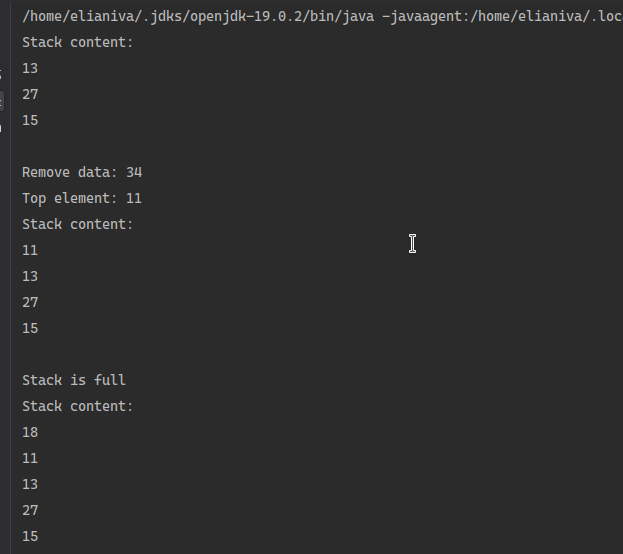
\includegraphics[width=.5\textwidth]{./images/q1-2-output.png}
            \caption{The output after adding 18 and 40}
        \end{figure}
    }
    \item {
        In previous number, the data inserted in to the stack is only 18, and 40 is not inserted. Why is that?

        Because the maximum capacity is 5 and 40 is the 6th item which means that it can no longer contain the new item.
    }
\end{enumerate}

\section{Lab Activity}
\subsection{Questions}
\begin{enumerate}
    \item {
        In class \texttt{StackMain}, when calling \texttt{push()} method, the argument is \texttt{bk}.
        What information is included in the \texttt{bk} variable?

        The information included is the Book class that was constructed before passing it to the push method
    }
    \item {
        Which of the program that its usage is to define the capacity of the stack?

        It's in the constructor of the Stack, the constructor receives an integer that defines the size of the stack.
    }
    \item {
        What is the function of do-while that exists in \texttt{StackMain} class?

        It is used to repeat the process of inserting the book into the stack until the user no longer wants to continue.
    }
    \item {
        Modify the program in \texttt{StackMain}, so that the user may choose which operation (push, pop, peek, print) to do in stack from program menu!
    }
\end{enumerate}

\section{Lab Activity}
\subsection{Questions}
\begin{enumerate}
    \item {
        Please explain the flow of method in \texttt{Postfix} class!
        
        \begin{itemize}
            \item \texttt{push} - add an item to the top of the stack, and increment the top counter
            \item \texttt{pop} - removes the top-most item from the stack, and decrement the top counter
            \item \texttt{degree} - gets the order of precedence for each operator using switch case
            \item \texttt{isOperand} - checks if its an operand or not by checking if the character is within the range of A-Z, a-z, and 0-9
            \item \texttt{isOperator} - checks if its an operator or not by checking if the character is a mathematical operator
            \item {
                \texttt{convert}
                
                It walks through every character of the input, every operand is inserted into the postfix string. 
                Everytime it encounters an operator, it pushes it to the stack.
                However, if there is an operator with higher precedence in the stack, it will pop that operator first and then put the curren toperator into the stack.
                If it encounters a closing brackets, it will pop every items inside the stack until it found the opening brace.
            }
        \end{itemize}
    }
    \item {
        What is the function of this program code?

        \begin{minted}[autogobble,fontsize=\small]{java}
            c = Q.charAt(i);
        \end{minted}

        It is used to get the character at position i
    }
    \item {
        Execute the program again, how's the result if we insert \textbf{3*5\^{}(8-6)\%3} for the expression?

        The result is \textbf{3586-\^{}3\%*}
    }
    \item {
        In $2^{nd}$ number, why the braces are not displayed in conversion result? Please explain

        Because the braces are not necessary since the order of the operand and the operator is already correct so
        there is no need to include them in the postfix notation.
    }
\end{enumerate}

\section{Assignments}
\begin{enumerate}
    \item {
        Create a program with Stack implementation to insert a sentence and display the reversed version of the sentence as a result!

        \textbf{CharStack.java}
        \begin{minted}[autogobble,fontsize=\small]{java}
            public class CharStack {
                int top = -1;
                int size;
                char[] data;

                public CharStack(int size) {
                    data = new char[size];
                    this.size = size;
                }

                boolean isFull() {
                    return top == size - 1;
                }

                boolean isEmpty() {
                    return top == -1;
                }

                void push(char c) {
                    if (isFull()) {
                        System.out.println("Stack is already full");
                        return;
                    }

                    top++;
                    data[top] = c;
                }

                char pop() {
                    if (isEmpty()) {
                        System.out.println("Stack is already empty");
                        return '.';
                    }

                    char item = data[top];
                    top--;
                    return item;
                }
            }
        \end{minted}

        \textbf{Assignment1.java}
        \begin{minted}[autogobble,fontsize=\small]{java}
            import java.util.Scanner;

            public class Assignment1 {
                public static void main(String[] args) {
                    Scanner sc = new Scanner(System.in);
                    System.out.print("Insert the sentence: ");
                    String sentence = sc.nextLine();

                    CharStack charStack = new CharStack(sentence.length());
                    for (int i = 0; i < sentence.length(); i++) {
                        charStack.push(sentence.charAt(i));
                    }

                    System.out.print("Reversed sentence: ");
                    while (!charStack.isEmpty()) {
                        System.out.write(charStack.pop());
                    }
                    System.out.flush();
                }
            }
        \end{minted}
    }
    \item {
        Every Sunday, Dewi shops to a supermarket that is in her residential area. Everytime she
        finishes, she keeps the receipt of what she has bought in a wardrobe. After 2 months, She had 8 receipts.
        She plans to trade her 5 receipts in exchange for a voucher. Create a program using stack implementation
        to store Dewi's receipt. As well as the retrieving of the receipts. The information that are included in a receipt are as follow:

        \begin{itemize}
            \item Transaction ID
            \item Date
            \item Quantity of items
            \item Total price
        \end{itemize}

        \textbf{Code}

        \begin{itemize}
            \item {
                \texttt{Receipt.java}

                \begin{minted}[autogobble,fontsize=\small]{java}
                    public class Receipt {
                        String transactionId;
                        String date;
                        int quantity;
                        int totalPrice;

                        public Receipt(String transactionId, String date, int quantity, int totalPrice) {
                            this.transactionId = transactionId;
                            this.date = date;
                            this.quantity = quantity;
                            this.totalPrice = totalPrice;
                        }
                    }
                \end{minted}
            }
            \item {
                \texttt{ReceiptStack.java}

                \begin{minted}[autogobble,fontsize=\small]{java}
                    public class ReceiptStack {
                        int size;
                        int top;
                        Receipt[] data;

                        public ReceiptStack(int size) {
                            this.size = size;
                            data = new Receipt[size];
                            top = -1;
                        }

                        public boolean isEmpty() {
                            return top == -1;
                        }

                        public boolean isFull() {
                            return top == (size - 1);
                        }

                        public void push(Receipt book) {
                            if (isFull()) {
                                System.out.println("Stack is full");
                                return;
                            }

                            top++;
                            data[top] = book;
                        }

                        public void pop() {
                            if (isEmpty()) {
                                System.out.println("Stack is empty");
                                return;
                            }

                            Receipt x = data[top];
                            top--;
                            System.out.println("Remove data: " + x.transactionId + " " + x.date + " " + x.quantity + " " + x.totalPrice);
                        }

                        public void peek() {
                            System.out.println("Top element: " + data[top]);
                        }

                        public void print() {
                            System.out.println("Stack content: ");
                            for (int i = top; i > -1; i--) {
                                System.out.println(data[i].transactionId + " " + data[i].date + " " + data[i].quantity + " " + data[i].totalPrice);
                            }
                            System.out.println();
                        }

                        public void clear() {
                            if (isEmpty()) {
                                System.out.println("Failed! Stack is empty");
                                return;
                            }

                            top = -1;
                            System.out.println("Stack is now empty");
                        }
                    }
                \end{minted}
            }            
            \item {
                \texttt{ReceiptMain.java}

                \begin{minted}[autogobble,fontsize=\small]{java}
                    public class ReceiptMain {
                        public static void main(String[] args) {
                            ReceiptStack receiptStack = new ReceiptStack(10);

                            // adding 8 receipts
                            receiptStack.push(new Receipt("T001", "01-02-2022", 1, 2000));
                            receiptStack.push(new Receipt("T002", "05-02-2022", 2, 12000));
                            receiptStack.push(new Receipt("T003", "07-03-2022", 3, 9000));
                            receiptStack.push(new Receipt("T004", "09-04-2022", 7, 8000));
                            receiptStack.push(new Receipt("T005", "11-04-2022", 5, 4500));
                            receiptStack.push(new Receipt("T006", "12-05-2022", 4, 15000));
                            receiptStack.push(new Receipt("T007", "14-05-2022", 6, 7000));
                            receiptStack.push(new Receipt("T008", "24-07-2022", 9, 8200));

                            // display items
                            receiptStack.print();

                            // pop 5 receipts
                            for (int i = 0; i < 5; i++) {
                                receiptStack.pop();
                            }
                            System.out.println();

                            // display receipts
                            receiptStack.print();
                        }
                    }
                \end{minted}
            }
        \end{itemize}
        \pagebreak
        \textbf{Output}
        \begin{figure}[h]
            \centering
            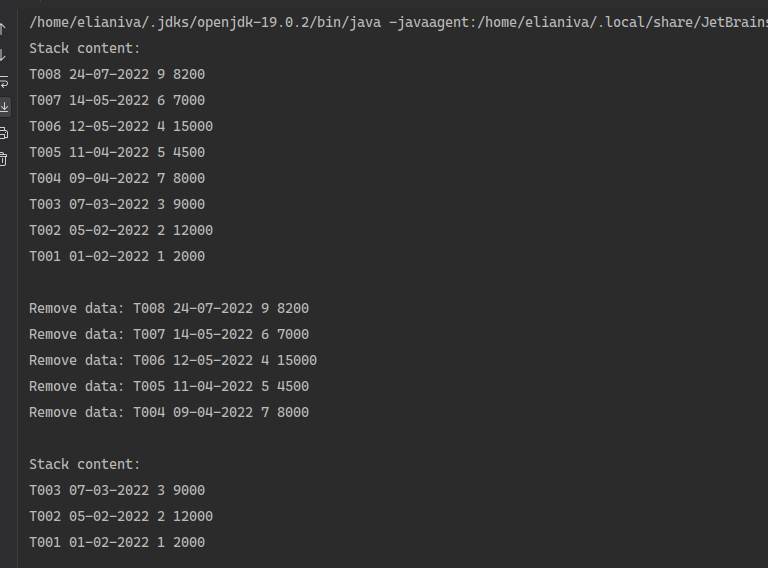
\includegraphics[width=.6\textwidth]{./images/assignment-output.png}
        \end{figure}
    }
\end{enumerate}

\end{document}

